
%%%%%%%%%%%%%%%%%%%%%%%%%%%%%%%%%%%%%%%%%%%%%%%%%%%%%%%%
%%%%%%%%%%%%%%%%%%%%%DATASET 1%%%%%%%%%%%%%%%%%%%%%%%%%%%%
\begin{figure}[h!]
    \centering
    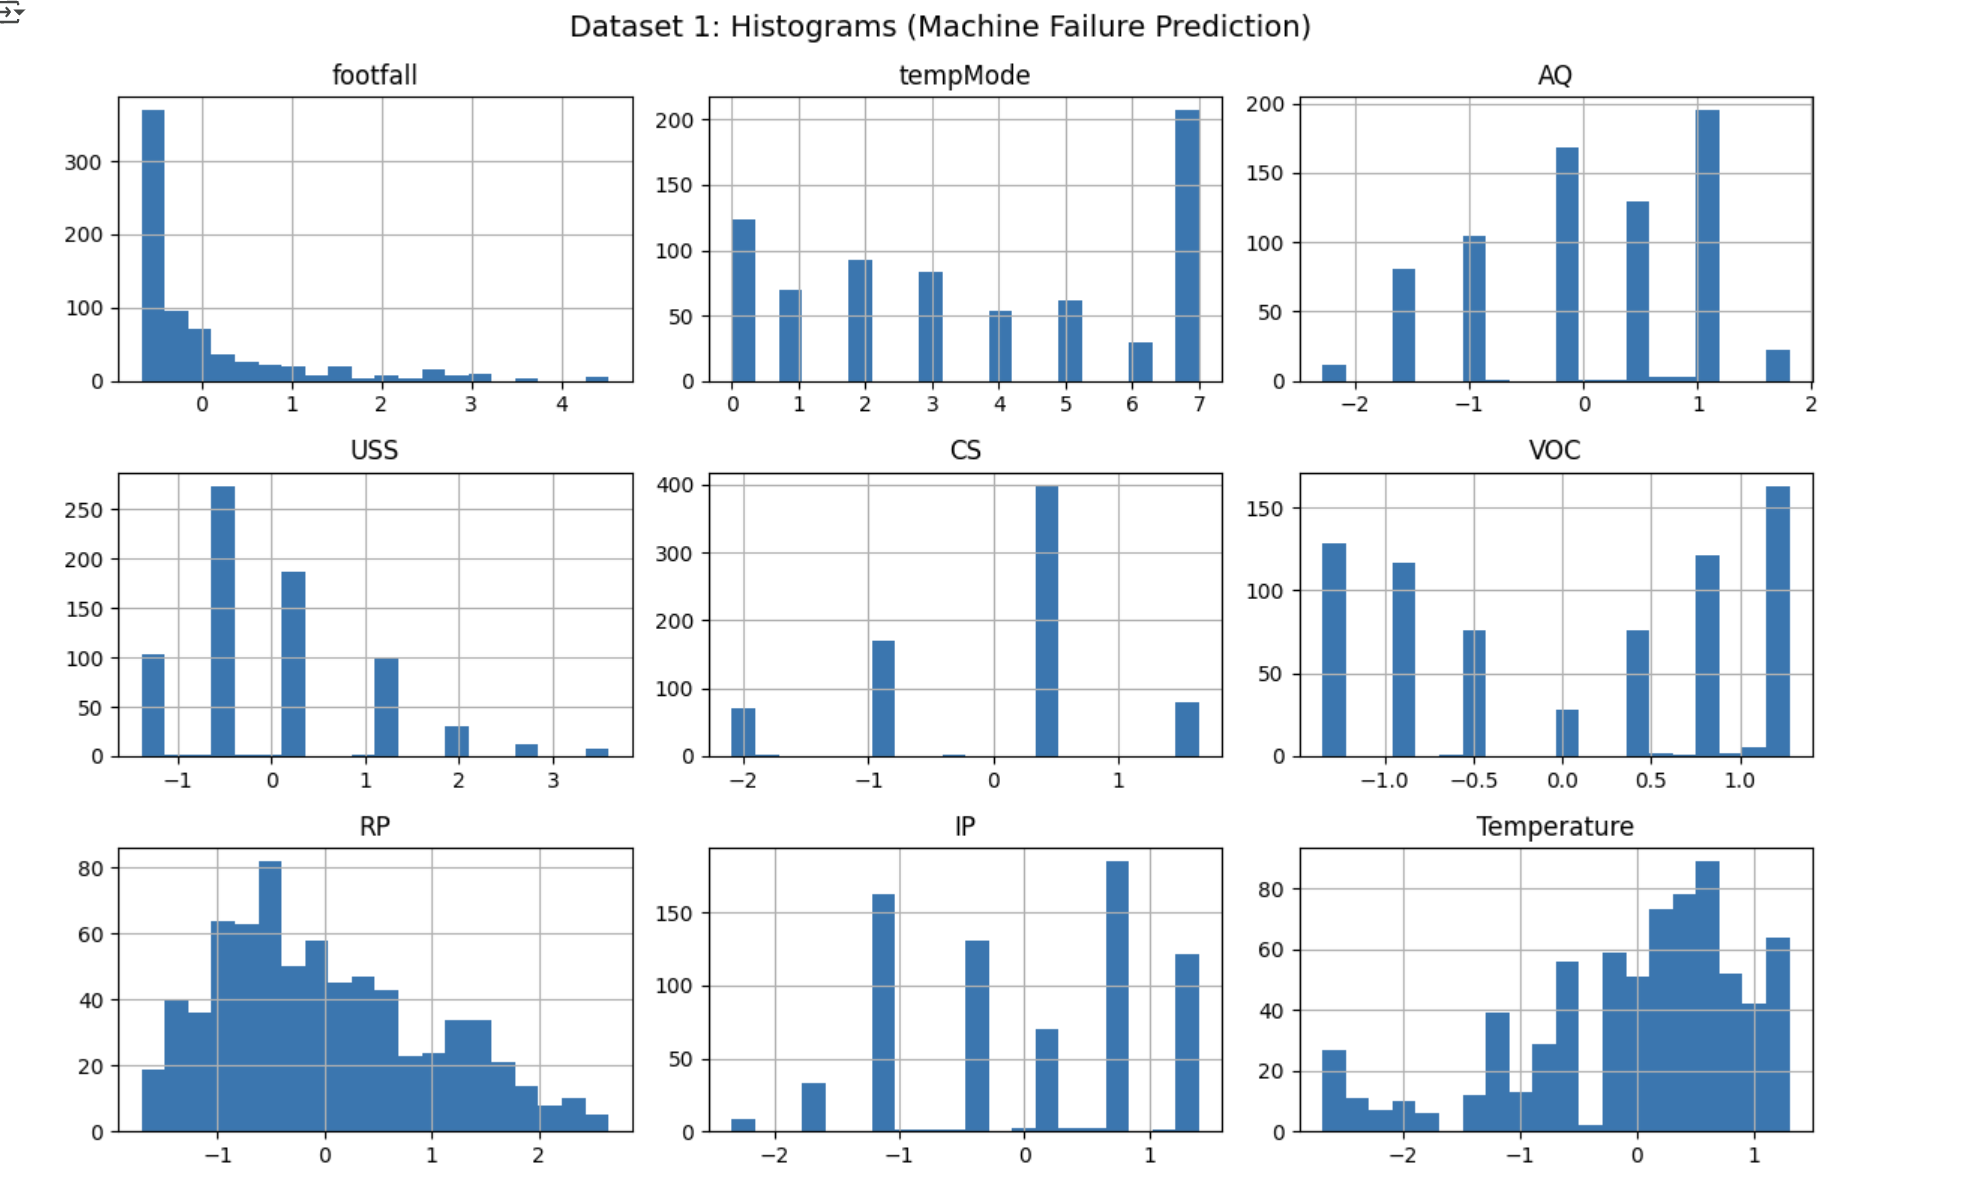
\includegraphics[width=0.8\textwidth]{figures/dataset 1/dataset1_hist.png}
    \caption{Histograms for Dataset 1}
    \label{fig:histograms_dataset1}
\end{figure}

\begin{figure}[h!]
    \centering
    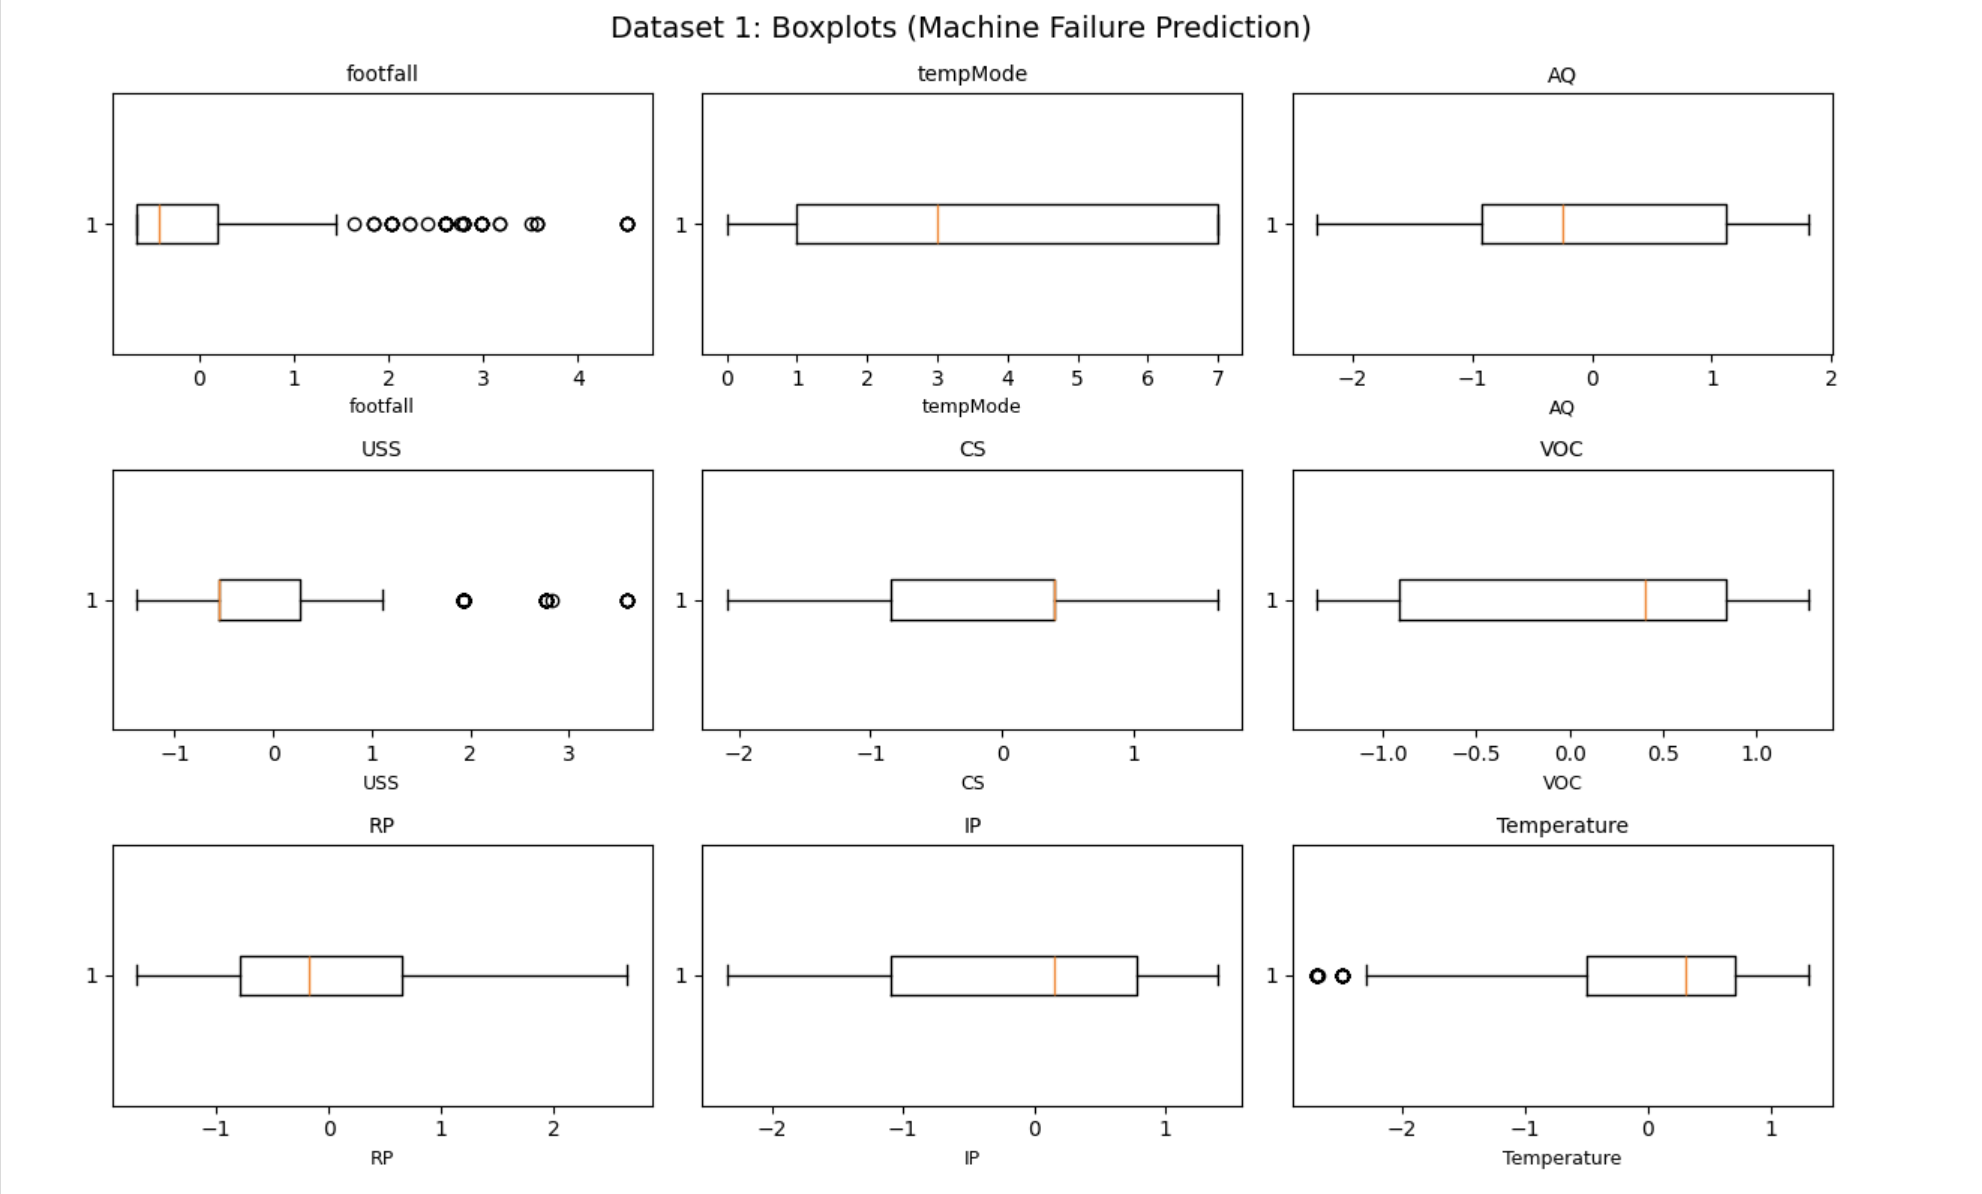
\includegraphics[width=0.8\textwidth]{figures/dataset 1/dataset1_box.png}
    \caption{Boxplots for Dataset 2}
    \label{fig:boxplot_dataset1}
\end{figure}

\begin{figure}[h!]
    \centering
    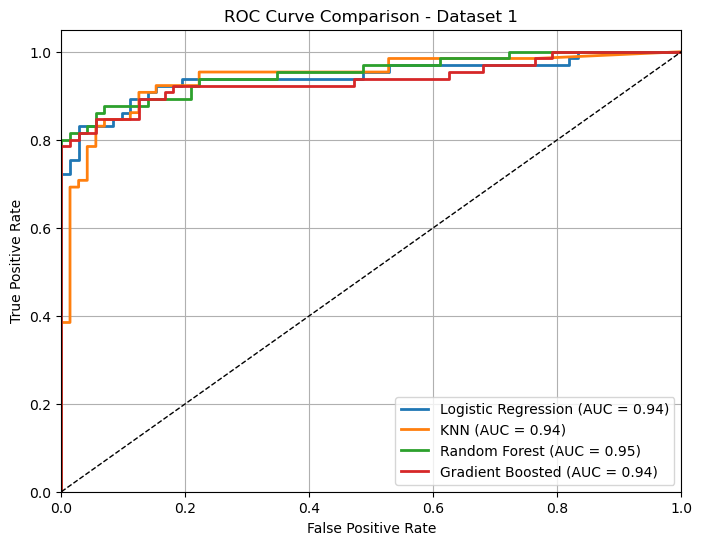
\includegraphics[width=0.8\textwidth]{figures/dataset 1/dataset1_all_models.png}
    \caption{Model Comparison for Dataset 1}
    \label{fig:all_models_dataset1}
\end{figure}

\begin{figure}[h!]
    \centering
    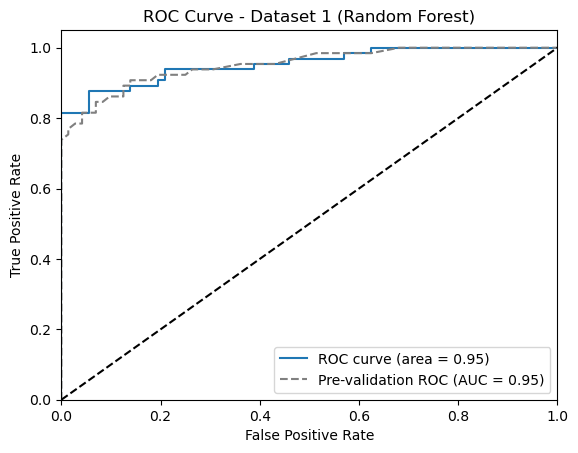
\includegraphics[width=0.8\textwidth]{figures/dataset 1/Dataset1-ROC_curve.png}
    \caption{ROC Curve Comparison for Dataset 1}
    \label{fig:roc_dataset1}
\end{figure}

\begin{figure}[h!]
    \centering
    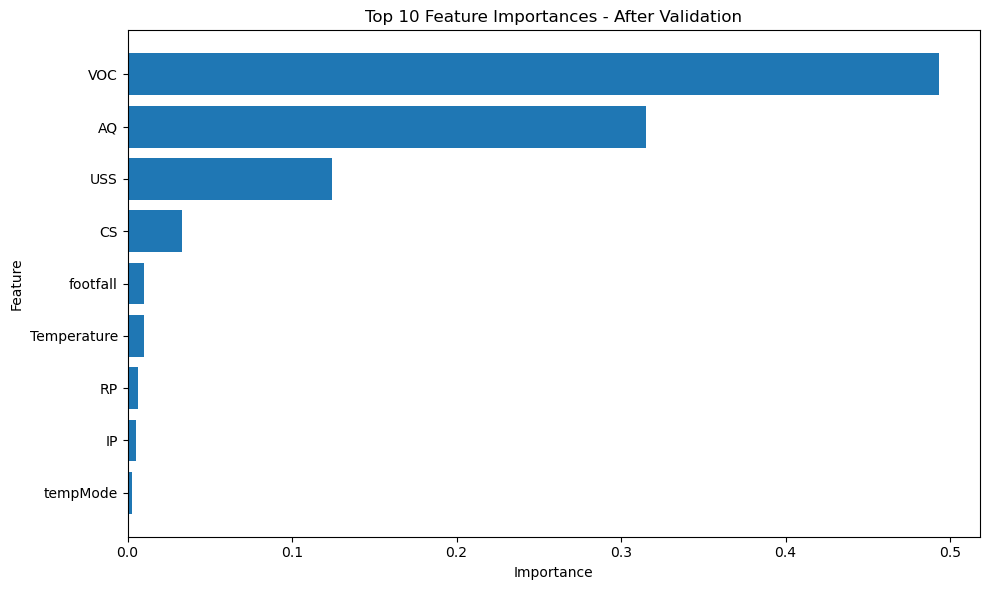
\includegraphics[width=0.8\textwidth]{figures/dataset 1/dataset1_feature_importance.png}
    \caption{Feature importance for Dataset 1}
    \label{fig:feature_importance_dataset1}
\end{figure}

\begin{figure}[h!]
    \centering
    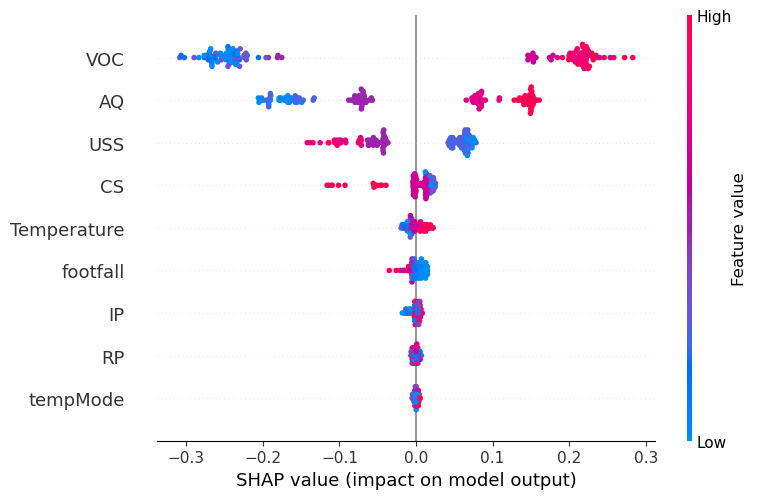
\includegraphics[width=0.8\textwidth]{figures/dataset 1/dataset1_shap_analysis.png}
    \caption{SHAP analysis for Dataset 1}
    \label{fig:shap_analysis_dataset1}
\end{figure}

\begin{figure}[h!]
    \centering
    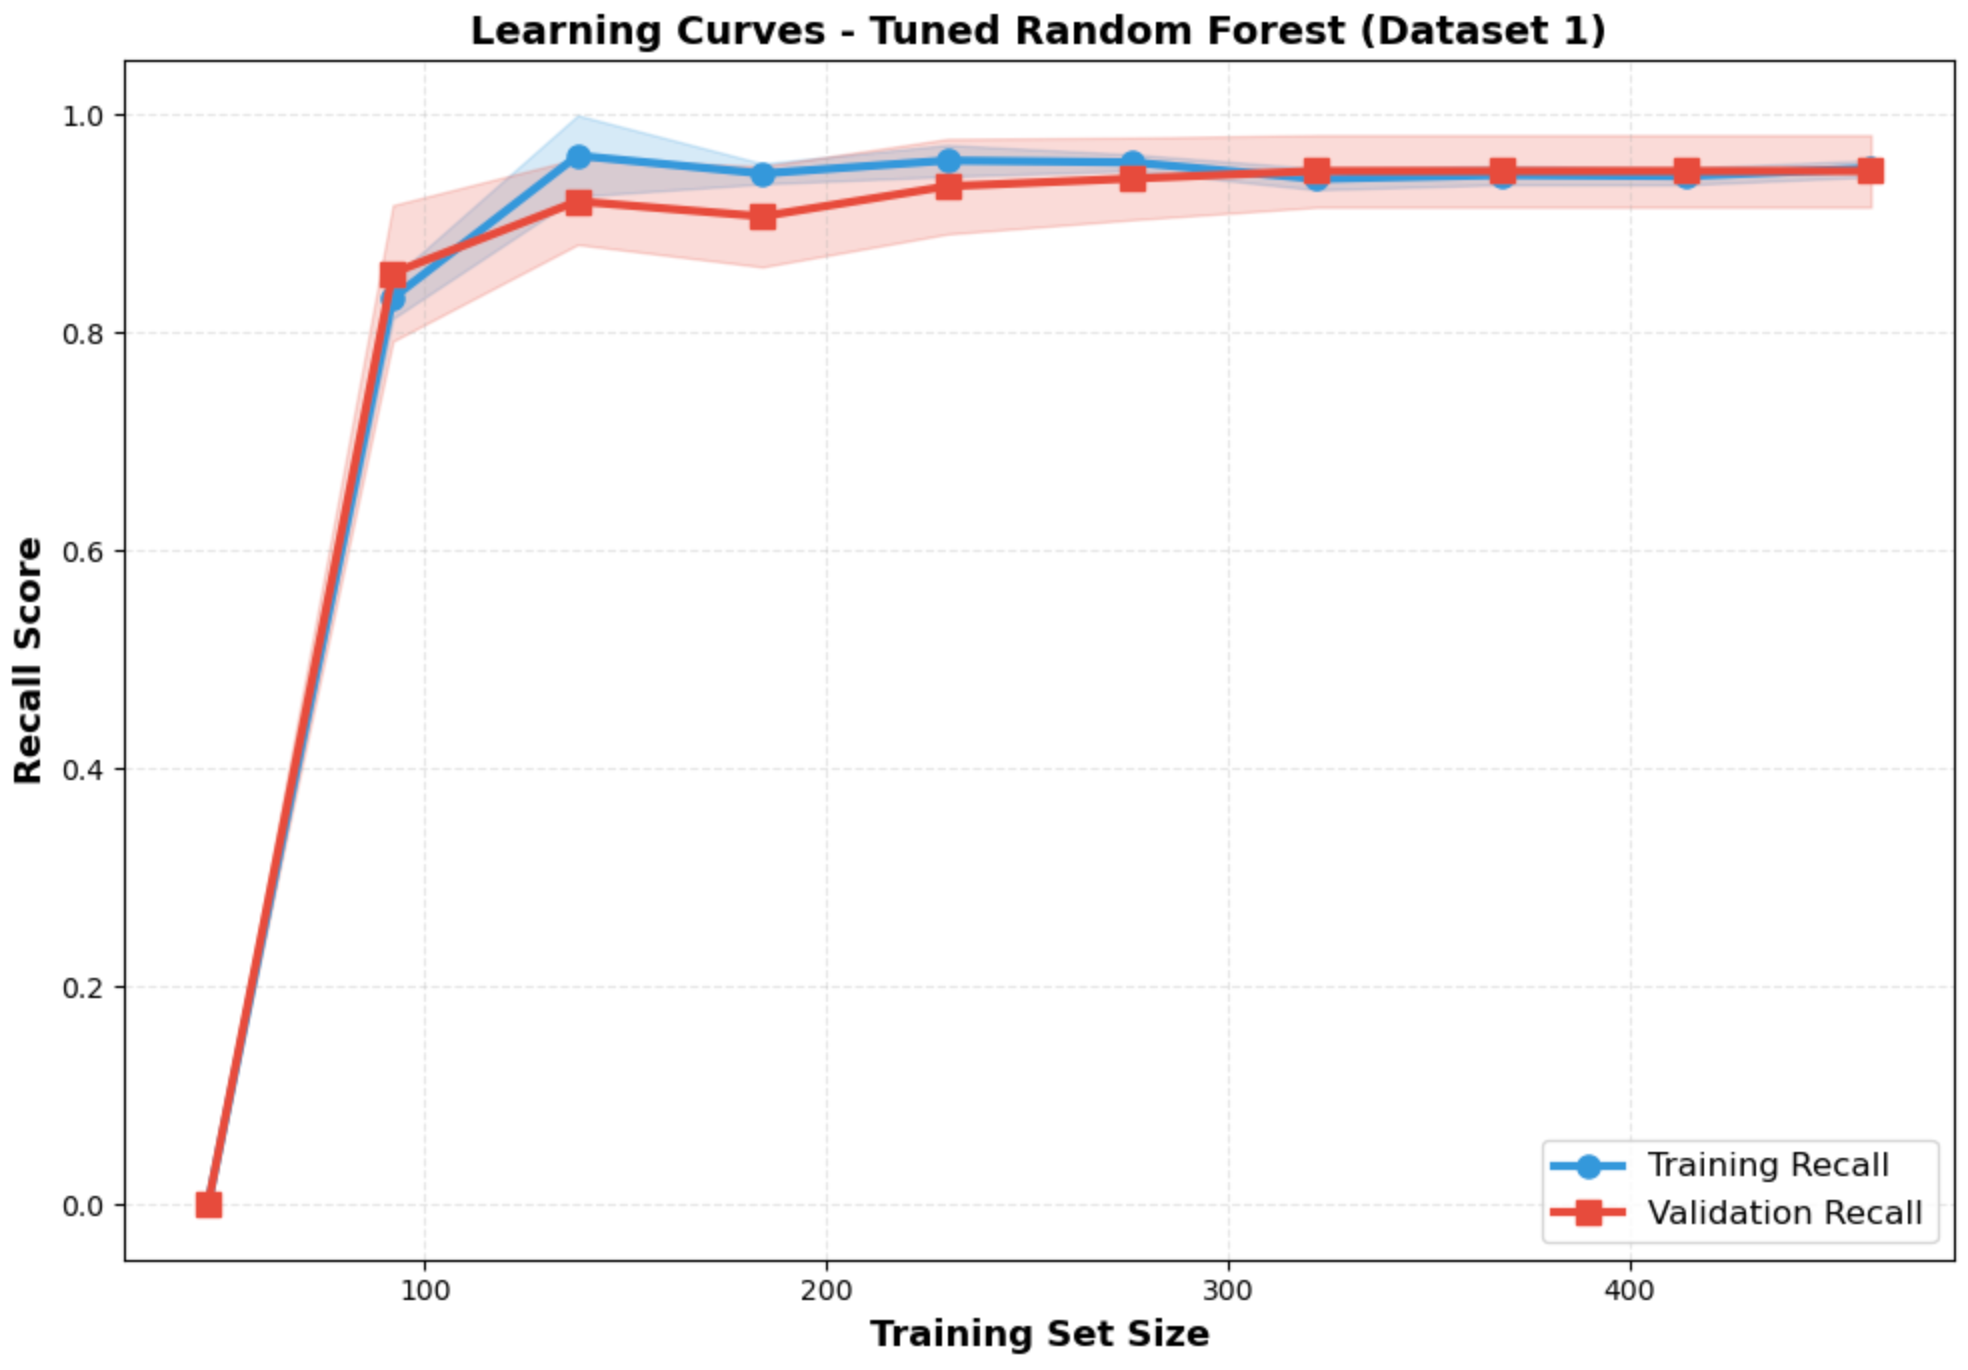
\includegraphics[width=0.8\textwidth]{figures/dataset 1/Dataset1-Learning_Curve.png}
    \caption{Learning Curve Comparison for Dataset 1}
    \label{fig:learning_curve_dataset1}
\end{figure}


%%%%%%%%%%%%%%%%%%%%%%%%%%%%%%%%%%%%%%%%%%%%%%%%%%%%%%%%
%%%%%%%%%%%%%%%%%%%%%%%%%DATASET 2%%%%%%%%%%%%%%%%%%%%%%

\begin{figure}[h!]
    \centering
    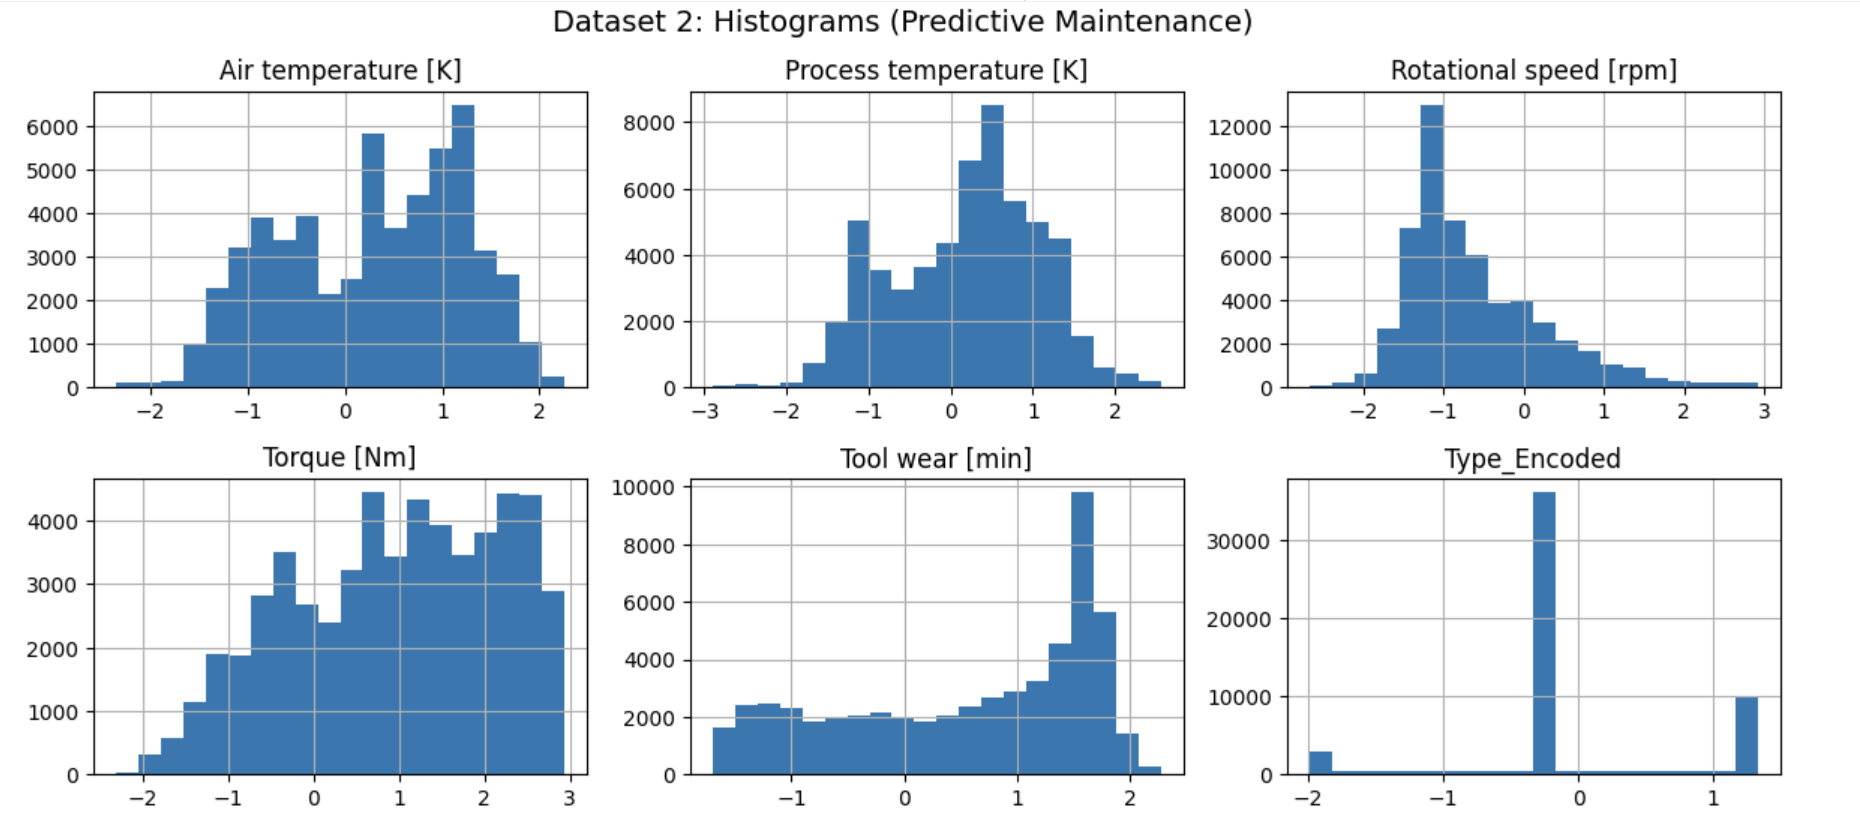
\includegraphics[width=0.8\textwidth]{figures/dataset 2/dataset2_hist.png}
    \caption{Histograms for Dataset 2}
    \label{fig:histograms_dataset2}
\end{figure}

\begin{figure}[h!]
    \centering
    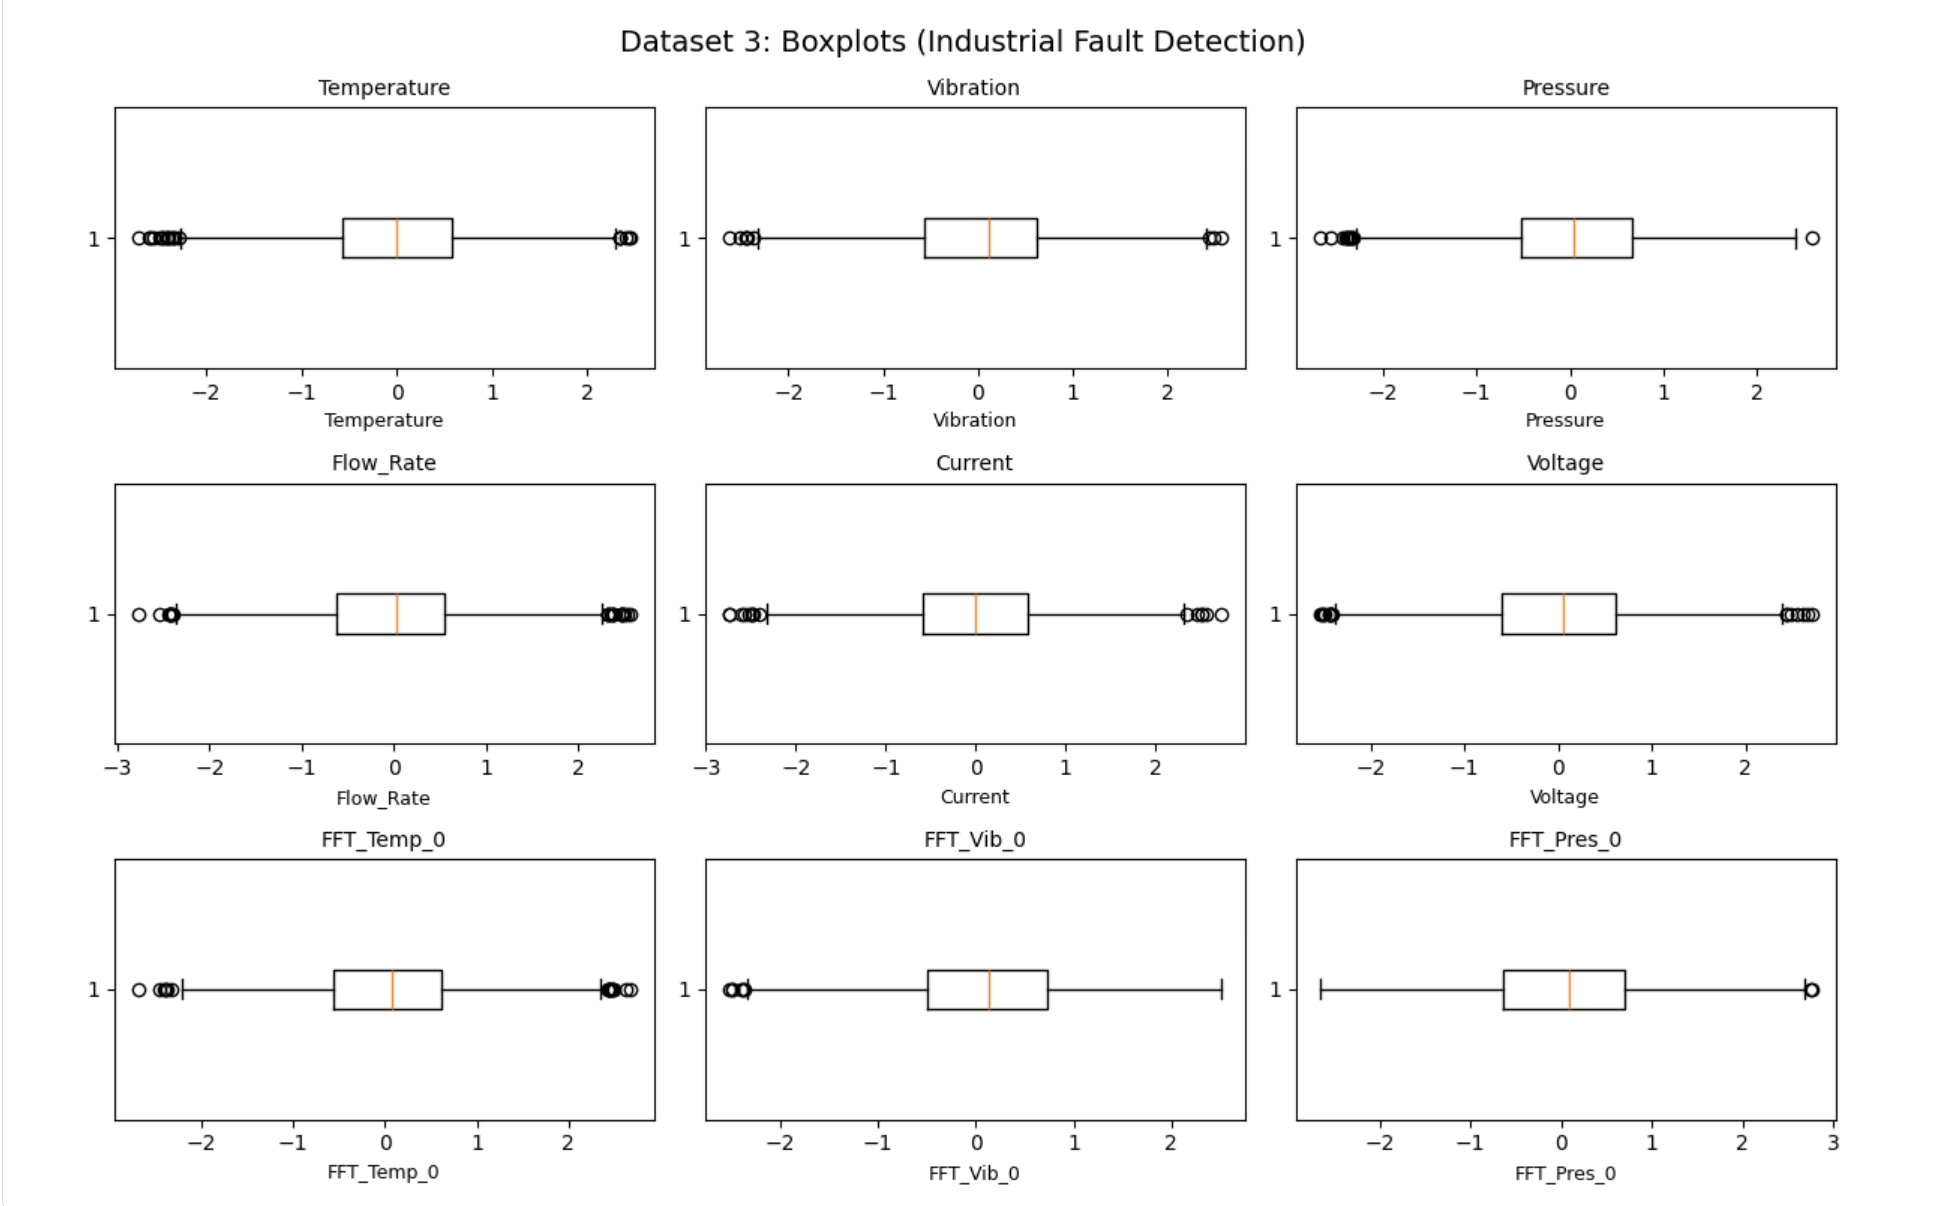
\includegraphics[width=0.8\textwidth]{figures/dataset 3/dataset3_box.png}
    \caption{Boxplots for Dataset 2}
    \label{fig:boxplot_dataset2}
\end{figure}

\begin{figure}[h!]
    \centering
    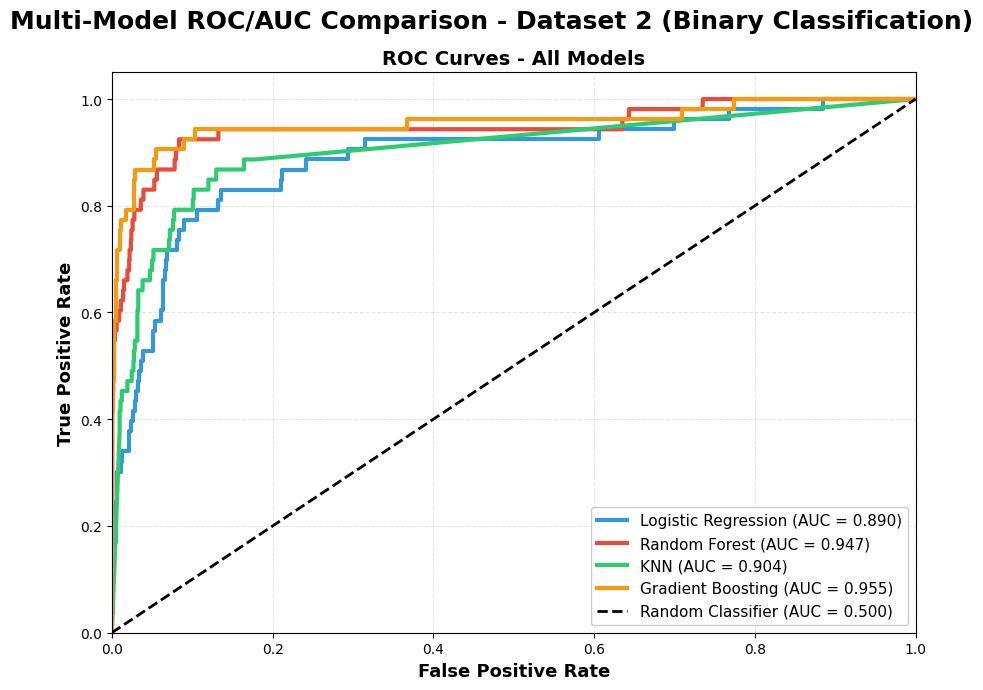
\includegraphics[width=0.8\textwidth]{figures/dataset 2/Dataset 2 multi-model comparison.png}
    \caption{Model Comparison for Dataset 2}
    \label{fig:all_models_dataset2}
\end{figure}

\begin{figure}[h!]
    \centering
    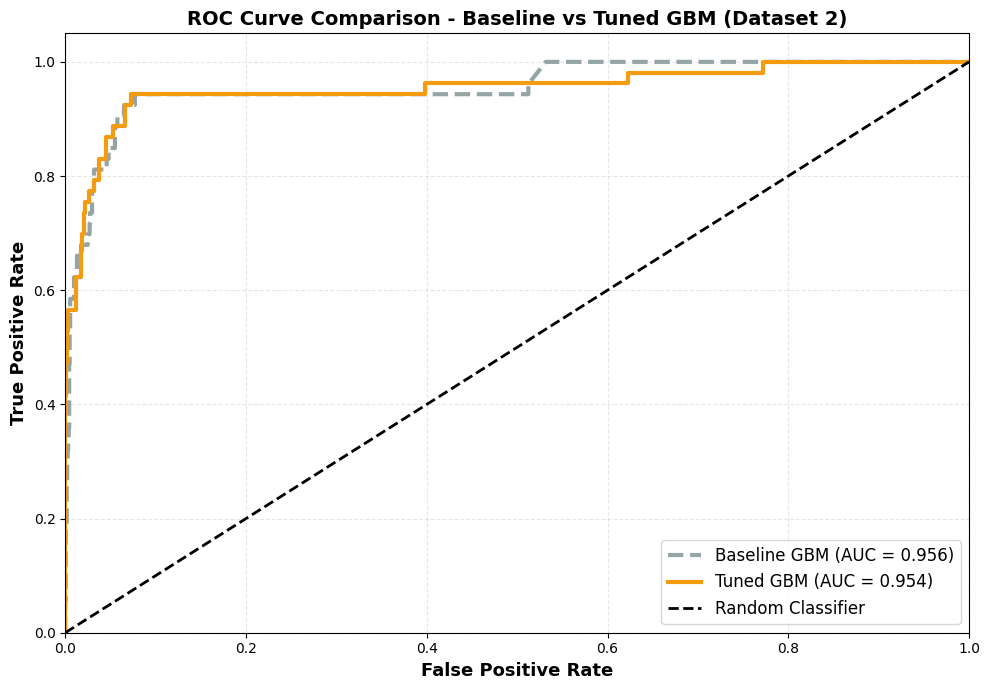
\includegraphics[width=0.8\textwidth]{figures/dataset 2/Dataset 2 baseline vs tuned.png}
    \caption{Baseline vs Tuned Model Comparison for Dataset 2}
    \label{fig:baseline_vs_tuned_dataset2}
\end{figure}

\begin{figure}[h!]
    \centering
    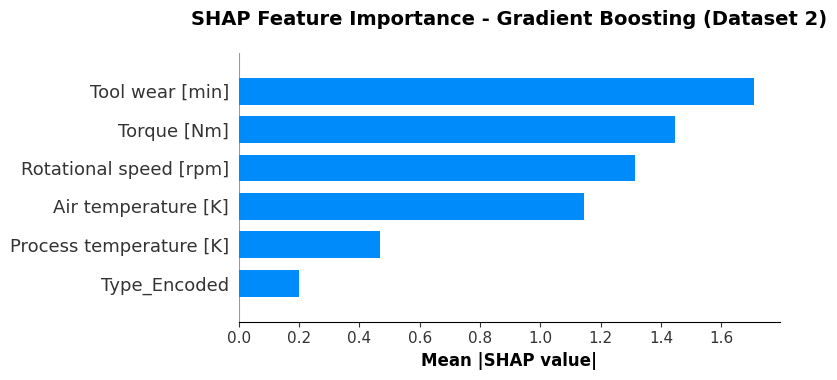
\includegraphics[width=0.8\textwidth]{figures/dataset 2/dataset 2 feature importance bar chart.png}
    \caption{Feature importance for Dataset 2}
    \label{fig:feature_importance_dataset2}
\end{figure}

\begin{figure}[h!]
    \centering
    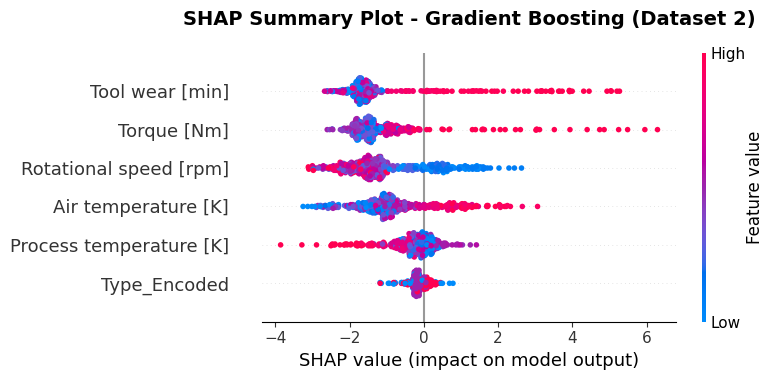
\includegraphics[width=0.8\textwidth]{figures/dataset 2/dataset 2 shap analysis.png}
    \caption{SHAP analysis for Dataset 2}
    \label{fig:shap_analysis_dataset2}
\end{figure}

\begin{figure}[h!]
    \centering
    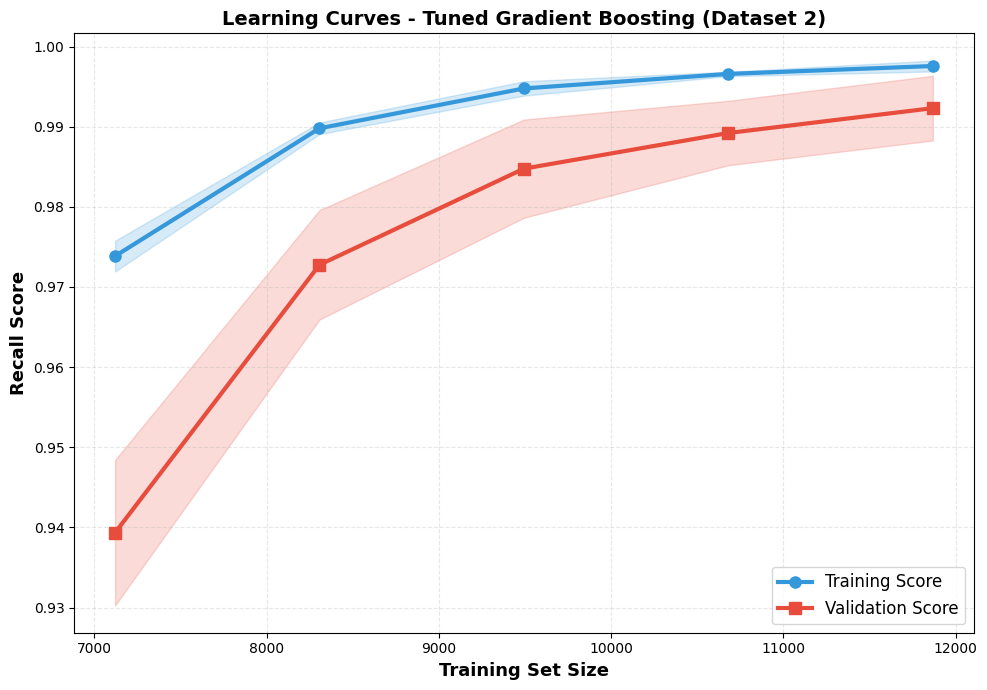
\includegraphics[width=0.8\textwidth]{figures/dataset 2/dataset 2 learning curve.png}
    \caption{Learning Curve Comparison for Dataset 2}
    \label{fig:learning_curve_dataset2}
\end{figure}



%%%%%%%%%%%%%%%%%%%%%%%%%%%%%%%%%%%%%%%%%%%%%%%%%%%%%%%%
%%%%%%%%%%%%%%%%%%%%%%%%%DATASET 3%%%%%%%%%%%%%%%%%%%%%%

\begin{figure}[h!]
    \centering
    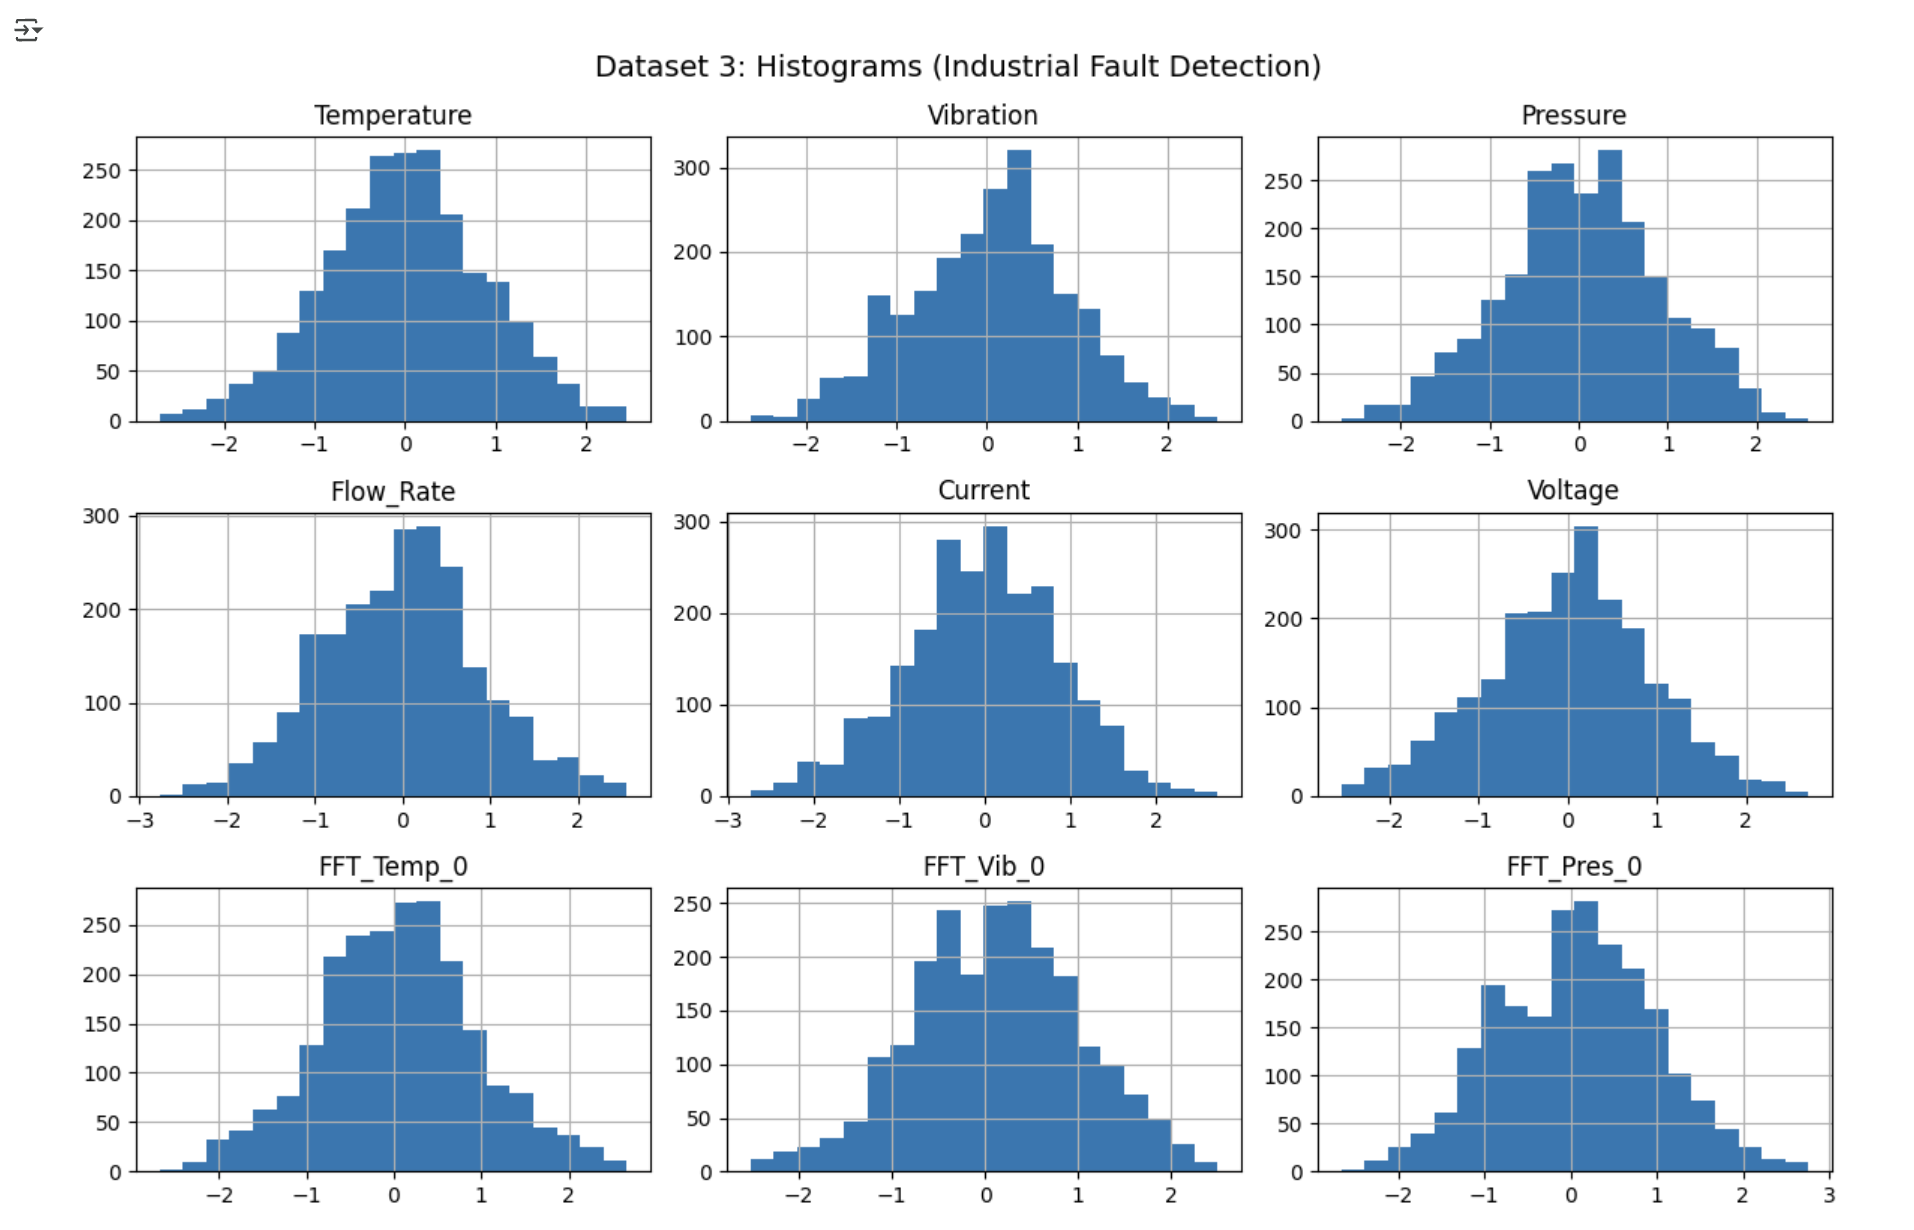
\includegraphics[width=0.8\textwidth]{figures/dataset 3/dataset3_hist.png}
    \caption{Histograms for Dataset 3}
    \label{fig:histograms_dataset3}
\end{figure}

\begin{figure}[h!]
    \centering
    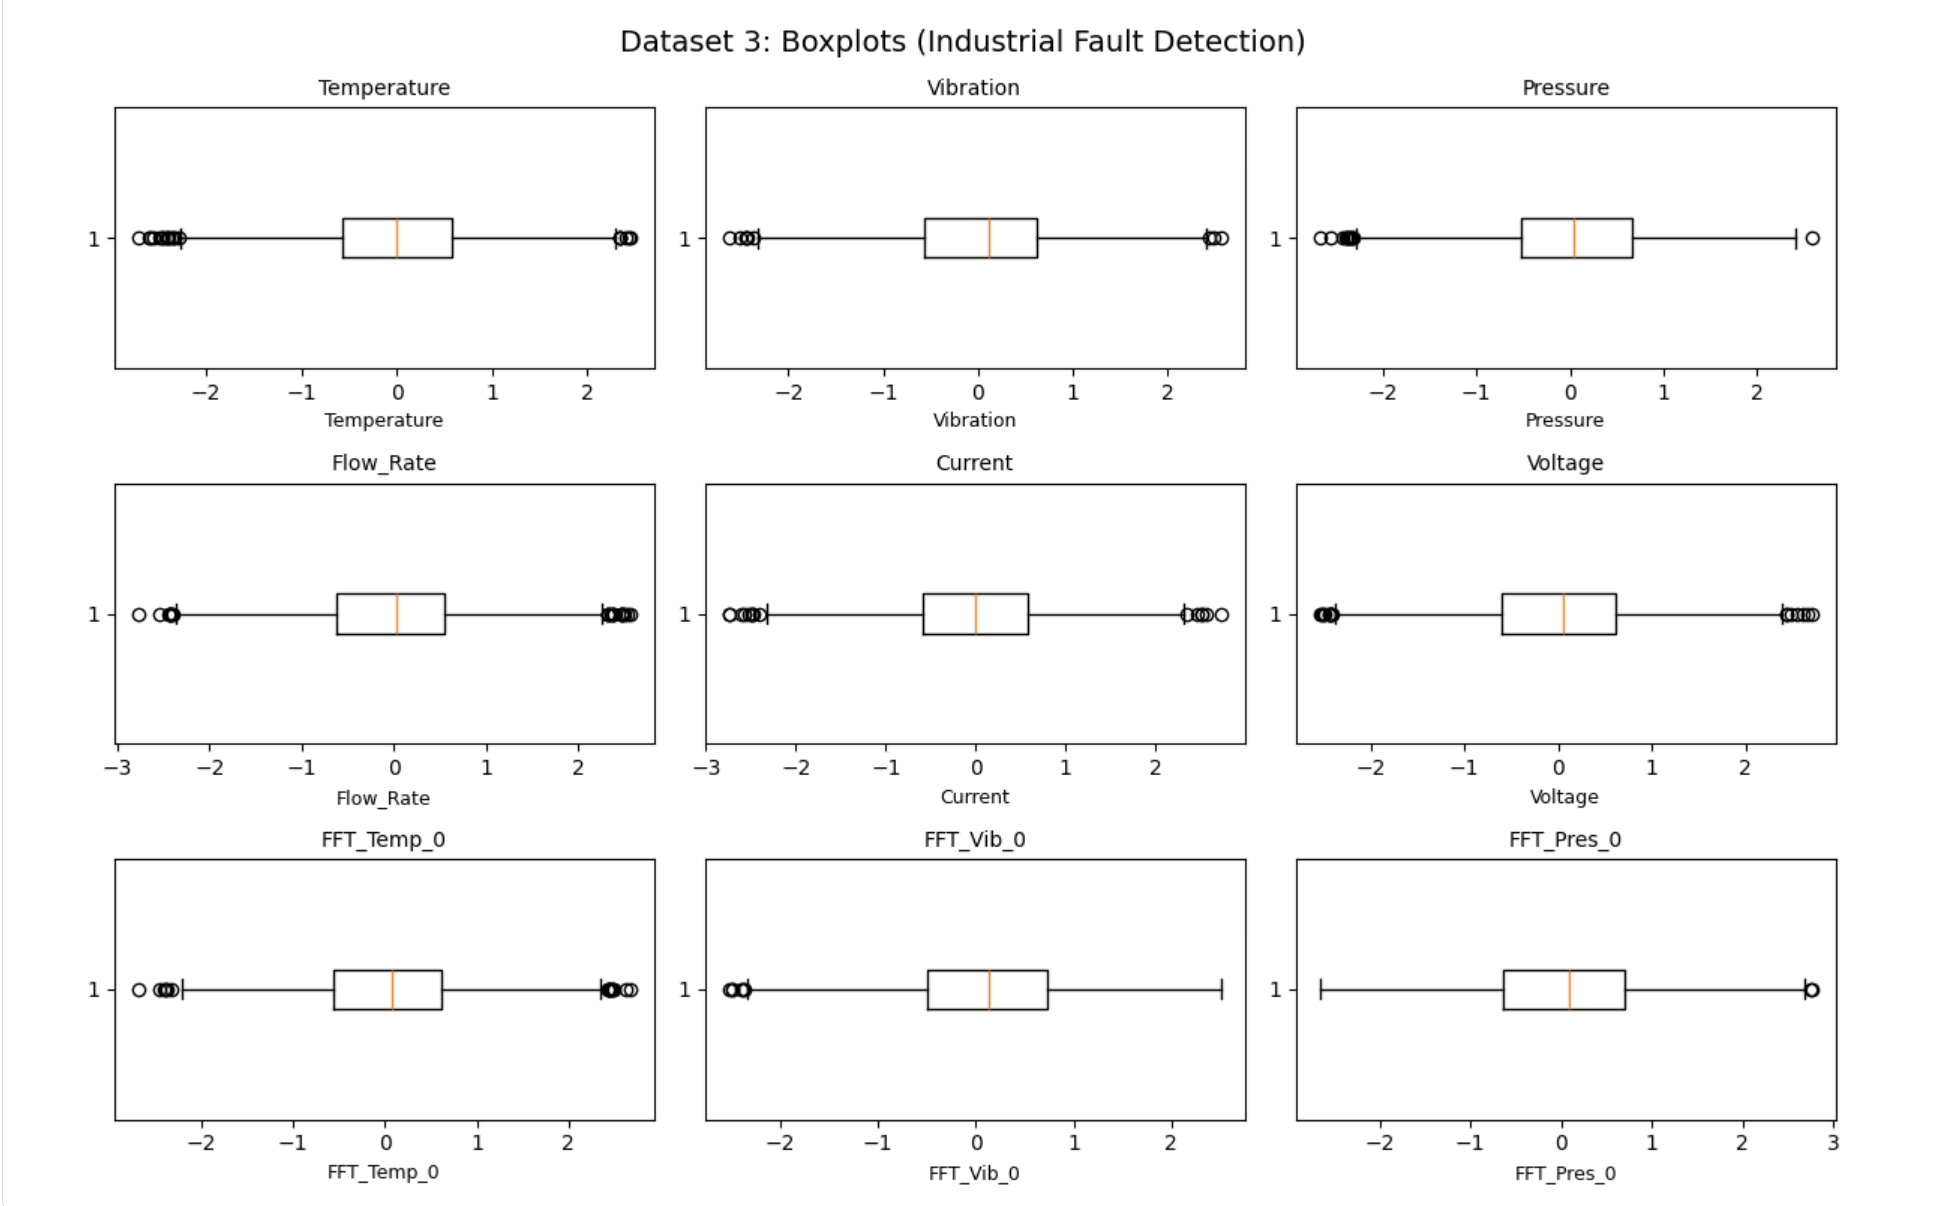
\includegraphics[width=0.8\textwidth]{figures/dataset 3/dataset3_box.png}
    \caption{Boxplots for Dataset 3}
    \label{fig:boxplot_dataset3}
\end{figure}

\begin{figure}[h!]
    \centering
    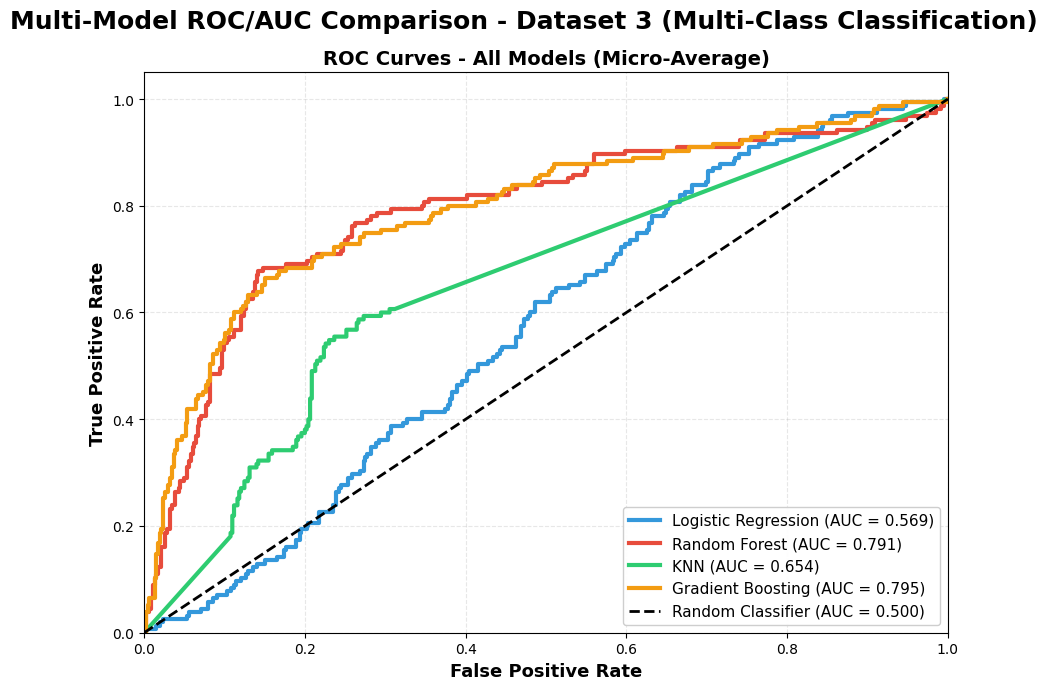
\includegraphics[width=0.8\textwidth]{figures/dataset 3/Dataset 3 multi-model comparison.png}
    \caption{Model Comparison for Dataset 3}
    \label{fig:all_models_dataset3}
\end{figure}

\begin{figure}[h!]
    \centering
    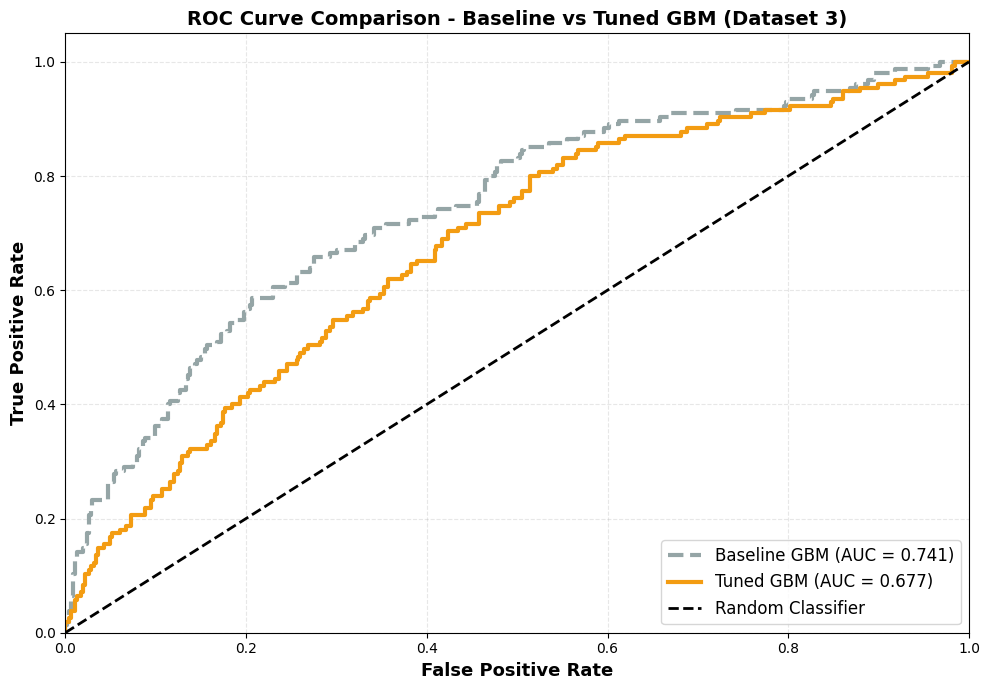
\includegraphics[width=0.8\textwidth]{figures/dataset 3/dataset 3 baseline vs tuned.png}
    \caption{Baseline vs Tuned Model Comparison for Dataset 3}
    \label{fig:baseline_vs_tuned_dataset3}
\end{figure}

\begin{figure}[h!]
    \centering
    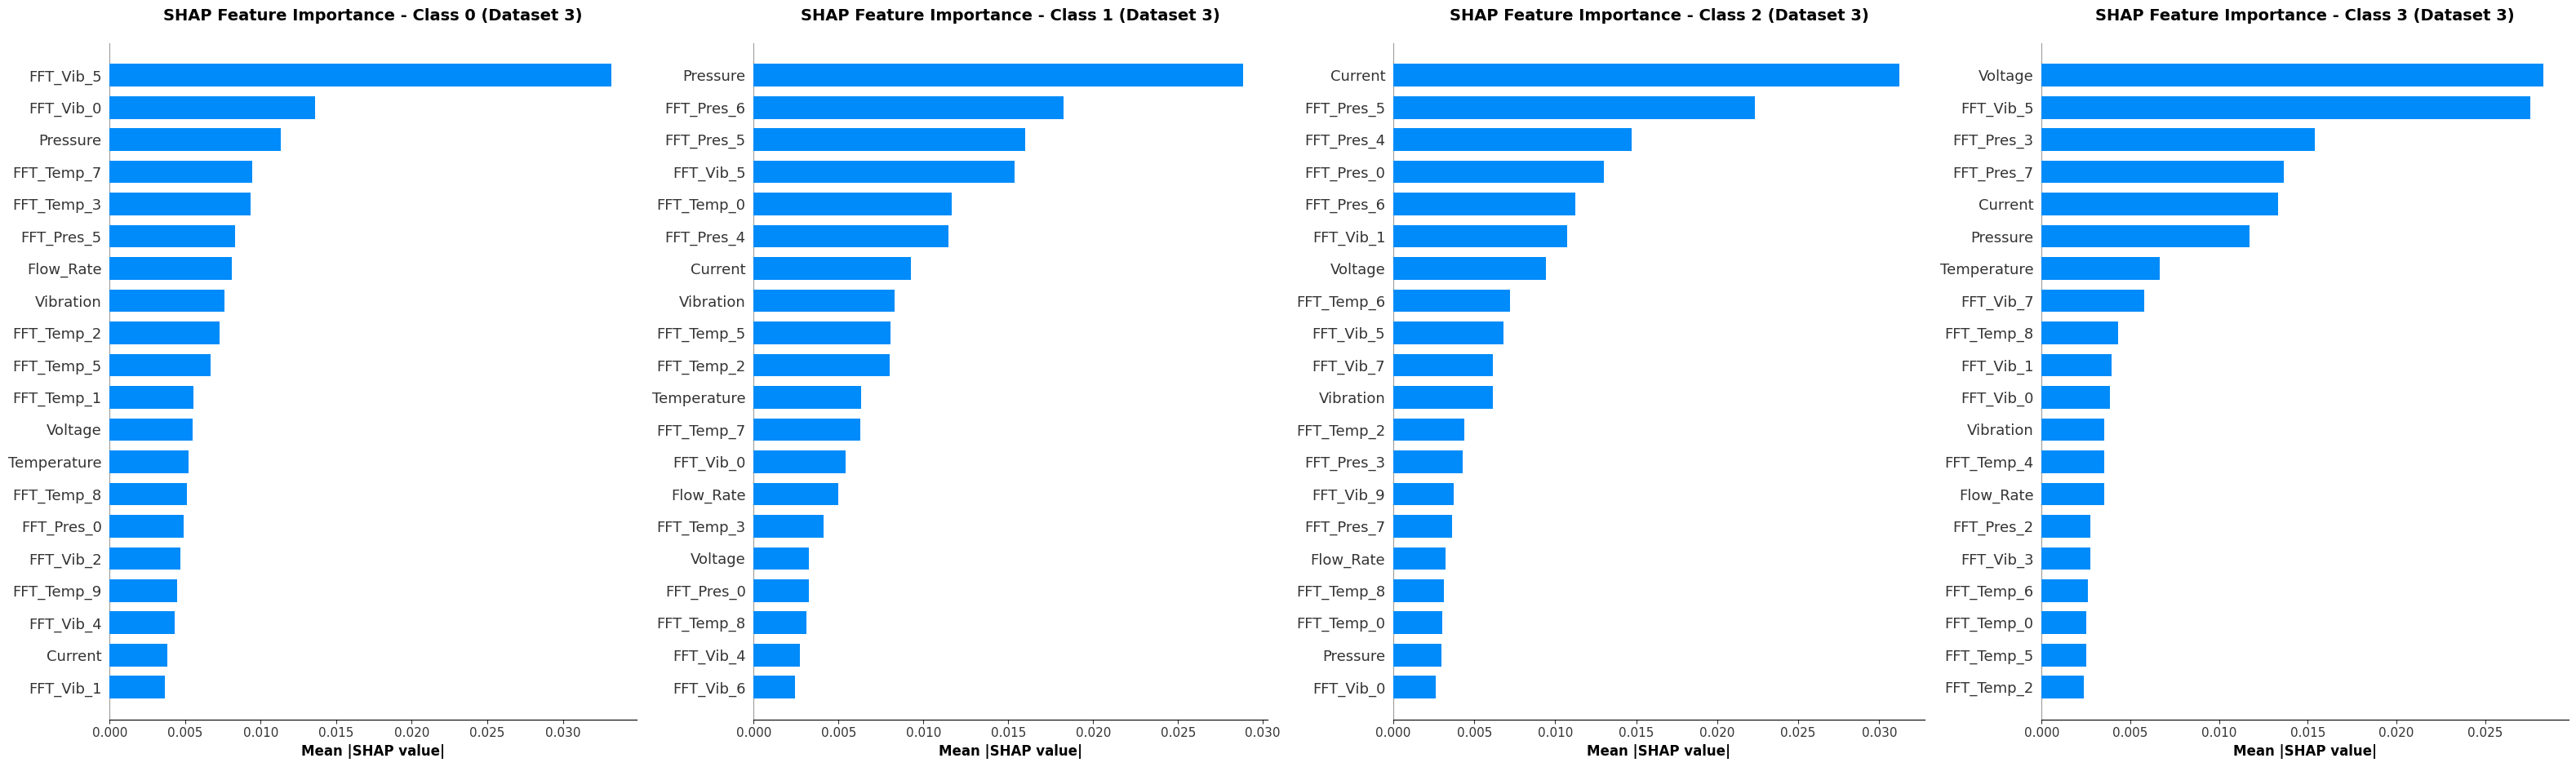
\includegraphics[width=0.8\textwidth]{figures/dataset 3/dataset 3 feature importance merged.jpg}
    \caption{Feature importance for Dataset 3}
    \label{fig:feature_importance_dataset3}
\end{figure}

\begin{figure}[h!]
    \centering
    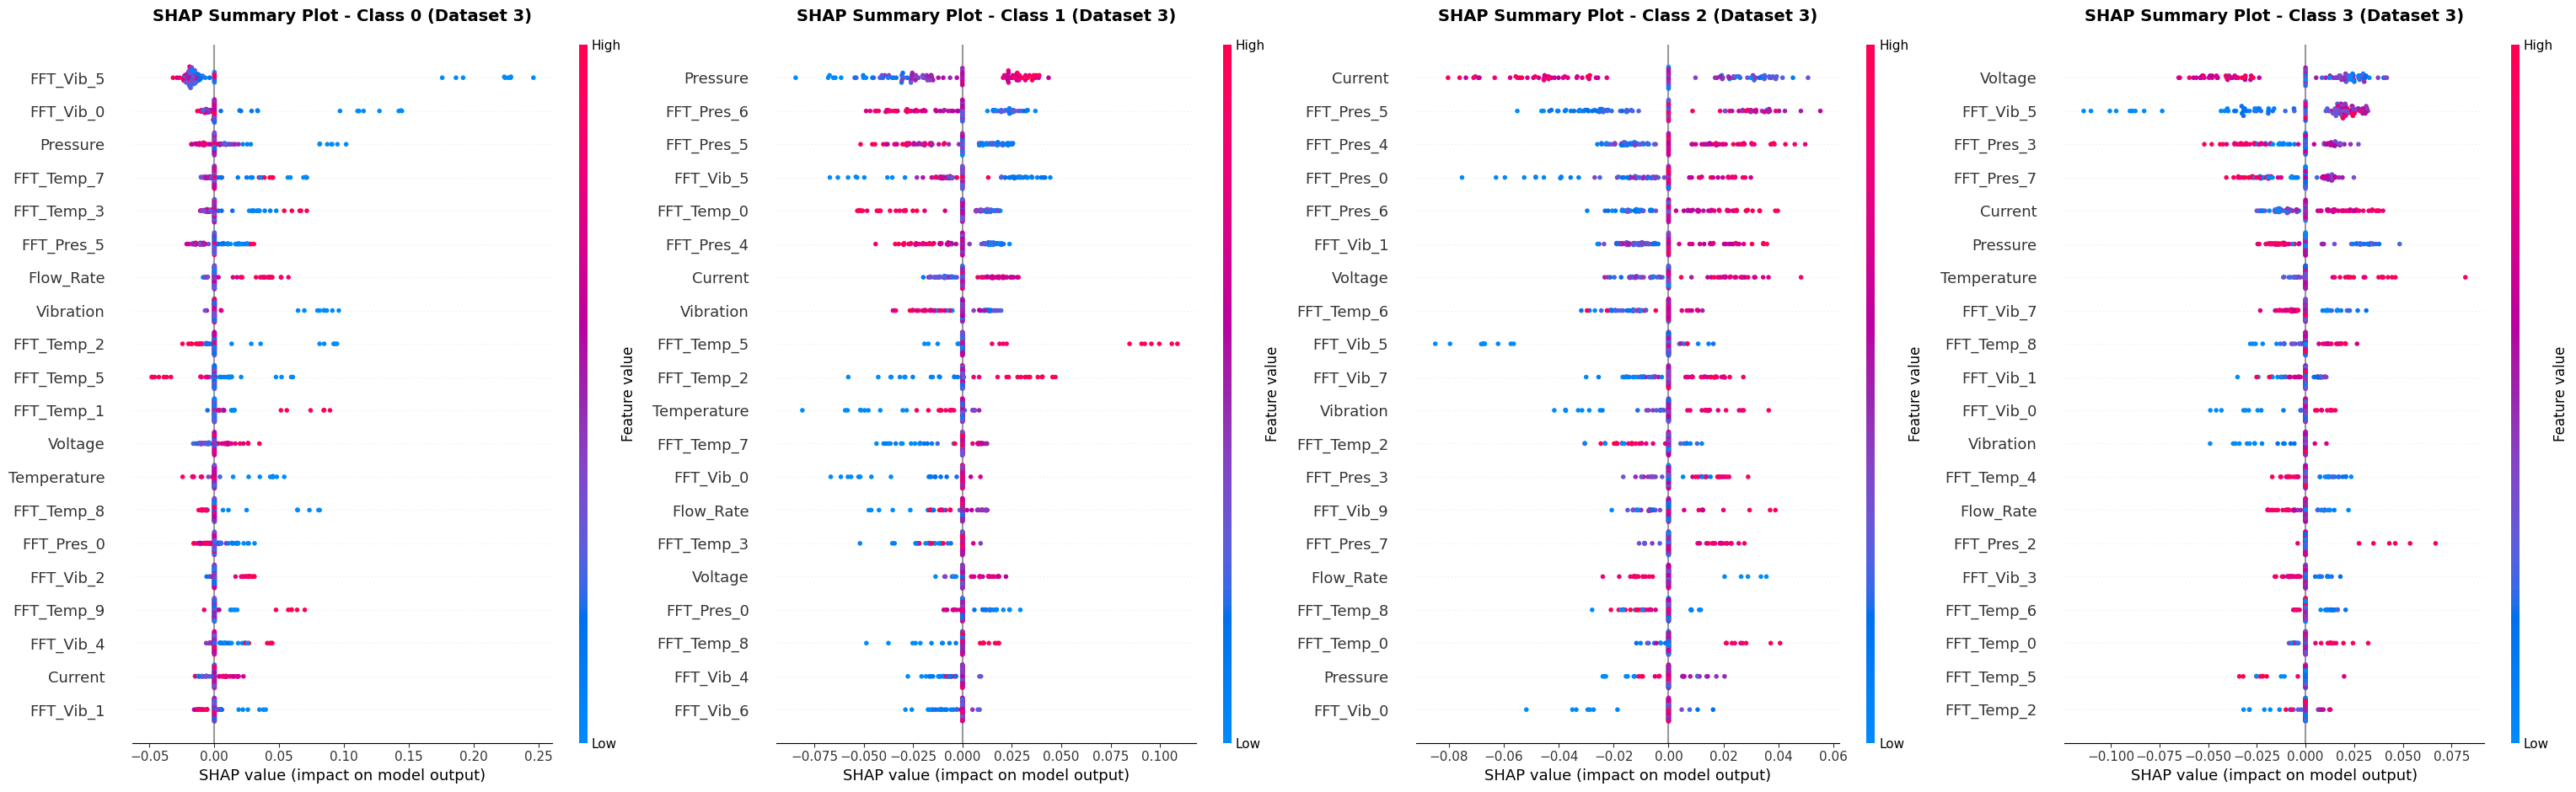
\includegraphics[width=0.8\textwidth]{figures/dataset 3/dataset 3 shap diagram merged.jpg}
    \caption{SHAP analysis for Dataset 3}
    \label{fig:shap_analysis_dataset3}
\end{figure}

\begin{figure}[h!]
    \centering
    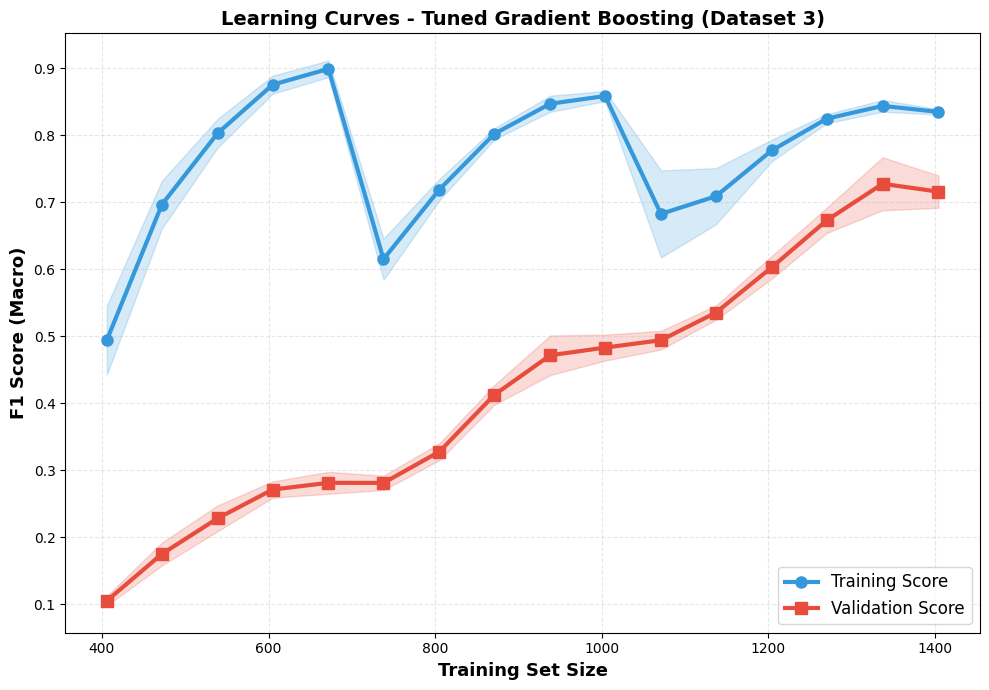
\includegraphics[width=0.8\textwidth]{figures/dataset 3/dataset 3 learning curve.png}
    \caption{Learning Curve Comparison for Dataset 3}
    \label{fig:learning_curve_dataset3}
\end{figure}


